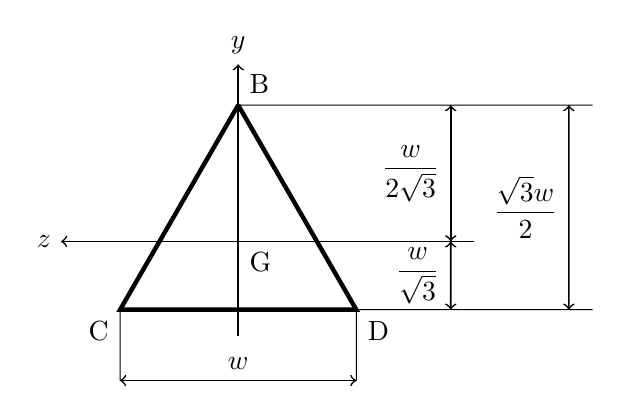
\begin{tikzpicture}[xscale=-3, yscale=3, ultra thick]
	%原点
	\draw (0, 0) node [below right]{G};
	%y軸
	\draw[semithick, ->] (0, -0.4)--(0, 0.75) node [above]{$y$};
	%z軸
	\draw[semithick, ->] (-1, 0)--(0.75, 0) node [left]{$z$};
	%頂点
	\path (0, 0.577) coordinate (B);
	\path (0.5, -0.289) coordinate (C);
	\path (-0.5, -0.289) coordinate (D);
	\draw (B) node [above right]{B};
	\draw (C) node [below left]{C};
	\draw (D) node [below right]{D};
	%辺
	\draw (B)--(C)--(D)--(B);
	%大きさ
	%
	\path (C)++(0, -0.3) coordinate (Cb);
	\draw[thin] (C)--(Cb);
	\path (D)++(0, -0.3) coordinate (Db);
	\draw[thin] (D)--(Db);
	\draw[semithick, <->] (Cb)--(Db);
	\draw (0, -0.589) node [above]{$w$};
	%
	\path (D)++(-0.4, 0) coordinate (Dr);
	\path (Dr)++(0, 0.289) coordinate (Or);
	\path (Dr)++(0, 0.866) coordinate (Br);
	\draw[semithick, <->] (Dr)--(Or);
	\draw[semithick, <->] (Or)--(Br);
	\path (Dr)++(0, 0.144) node [left]{$\displaystyle\frac{w}{\sqrt{3}}$};
	\path (Dr)++(0, 0.577) node [left]{$\displaystyle\frac{w}{2\sqrt{3}}$};
	%
	\path (D)++(-0.9, 0) coordinate (Drr);
	\path (Drr)++(0, 0.866) coordinate (Brr);
	\draw[semithick, <->] (Drr)--(Brr);
	\path (Drr)++(0, 0.433) node [left]{$\displaystyle\frac{\sqrt{3}w}{2}$};
	%
	\path (D)++(-1, 0) coordinate (Drrr);
	\path (Drrr)++(0, 0.866) coordinate (Brrr);
	\draw[thin] (D)--(Drrr);
	\draw[thin] (B)--(Brrr);
\end{tikzpicture}
